\documentclass{article}
\usepackage{microtype}
\usepackage{graphicx}
\usepackage{booktabs}
\usepackage{hyperref}
\usepackage{amsmath,amssymb}
\usepackage{algorithm}
\usepackage{algorithmic}
% ===========================================================================
% SUBMISSION MODE (do not change before submitting).
%
% ICML review is double blind. With the plain \usepackage{icml2026} below,
% icml2026.sty keeps \icmlshowauthors false, so the title block renders
% "Anonymous Authors", the affiliation becomes "Anonymous Institution", the
% correspondence line is replaced by a placeholder, and any notice passed to
% \printAffiliationsAndNotice is suppressed. Nothing in the block marked
% CAMERA-READY below can leak through, which is why the real author list is
% kept there rather than deleted.
%
% CAMERA-READY / PREPRINT. Two edits, and both are required:
%   1. \usepackage[accepted]{icml2026}   (or [preprint])
%   2. swap the two \ifdefined\isaccepted blocks below, i.e. comment out the
%      empty \icmlsetsymbol line and uncomment the one that defines the
%      equal-contribution symbol.
% Edit 2 matters: \@pa reads the symbol at every call even when authors are
% hidden, so leaving the symbol defined would print "Anonymous Authors*".
%
% When ICML 2027 releases its own style file, replace icml2026 in both places.
% ===========================================================================
\usepackage{icml2026}

\icmltitlerunning{Dynamics-Aware Gradient Clipping}
\begin{document}
\twocolumn[
\icmltitle{Dynamics-Aware Gradient Clipping: Protective Feedback for Unstable Training}

% Shared first authorship: Yuxin Li and Zisong Yuan contributed equally.
% \icmlsetsymbol is suppressed in submission mode (see the note above).
\ifdefined\isaccepted
  \icmlsetsymbol{equal}{*}
\else
  \icmlsetsymbol{equal}{}
\fi

\begin{icmlauthorlist}
% ---- SUBMISSION MODE -------------------------------------------------------
\icmlauthor{Anonymous Author(s)}{anon}
% ---- CAMERA-READY ONLY: comment out the line above, uncomment these two ----
% \icmlauthor{Yuxin Li}{equal,inst}
% \icmlauthor{Zisong Yuan}{equal,inst}
\end{icmlauthorlist}

% ---- SUBMISSION MODE -------------------------------------------------------
\icmlaffiliation{anon}{Anonymous Institution}
% ---- CAMERA-READY ONLY: real affiliation(s). Give each distinct institution
% ---- its own \icmlaffiliation and list its label in both \icmlauthor calls,
% ---- e.g. {equal,instA} and {equal,instB} for two separate institutions.
% \icmlaffiliation{inst}{FILL IN: Department, Institution, City, Country}
\icmlcorrespondingauthor{Anonymous Author(s)}{anonymous@example.com}
% ---- CAMERA-READY ONLY: corresponding author is Yuxin Li (placeholder email).
% \icmlcorrespondingauthor{Yuxin Li}{FILL.IN@example.com}
\vskip 0.3in
\begin{abstract}
Gradient clipping prevents destructive updates but a fixed threshold must be
retuned when the optimizer, learning rate, or model changes. We introduce
Dynamics-Aware Gradient Clipping (DAGC), a lightweight controller that changes
a global clipping threshold from the recent clipping exposure and gradient
alignment. An initial controller (DAGC-V1) drove the threshold in one direction
only: because its exposure term is non-negative for any exposure level, the
exposure alone could relax the threshold but could not tighten it. DAGC-V2 makes the same term bidirectional,
so realized exposure above a reference level lowers the threshold. We select V2
on separate development seeds and evaluate it with eight paired, held-out seeds
per method. On unstable FashionMNIST training with SGD, V2 improves over
calibrated fixed clipping by 0.82--2.18 percentage points across two learning
rates, and by 1.53 points on a different MLP architecture. On MNIST with a CNN
it improves by 1.16 points. It also exceeds adaptive gradient clipping (AGC) in
each condition. A sweep of the reference level from $0.1$ to $0.7$ leaves
accuracy unchanged to within $0.7$ points while realized exposure stays at the
ceiling throughout: what the correction buys is a threshold that can fall, not
the tracking of any particular exposure level. These are diagnostic-scale
MNIST-family experiments. Additional paired controls show that exposure removal
costs 5.47 points, while removing alignment costs only 0.16 points and a
calibration-derived open-loop schedule nearly matches V2. Thus the evidence
supports a protective threshold profile without establishing an additional
benefit from online directional feedback. The results establish a controlled signal rather
than broad large-scale generalization.
\end{abstract}
]

% This must come after the closing bracket of \twocolumn[...]. In submission
% mode the notice passed here is suppressed by icml2026.sty, so the shared
% first-authorship statement below cannot appear in a blind submission.
% CAMERA-READY: uncomment the \icmlEqualContribution line and drop the {} one.
\printAffiliationsAndNotice{}
% \printAffiliationsAndNotice{\icmlEqualContribution}

\section{Introduction}
Gradient clipping is a standard safeguard for exploding or destructive updates
\citep{pascanu2013difficulty}. In its usual global-norm form, however, the
threshold is constant throughout training. A threshold that is useful during a
transient spike can over-constrain later updates, whereas a permissive threshold
can fail in an unstable phase. This creates a per-setting tuning burden and
makes clipping behaviour difficult to transfer across learning rates and
architectures.

We study clipping as a feedback-control problem. DAGC maintains a scalar global
threshold and observes two signals already available in a training loop: whether
clipping was active and whether consecutive gradients agree in direction. Its
first version had a one-sided exposure response. Because $E_t\in[0,1]$,
the V1 exposure term $r(1-E_t)$ is non-negative at every exposure level, so the
exposure alone could only increase the threshold: even at maximal exposure it
merely slowed relaxation. The alignment term could still tighten the threshold,
but persistent clipping alone could not trigger that response. DAGC-V2 replaces
the term with $r(\tau-E_t)$, which changes sign, so excess exposure actively
lowers the threshold.

Our evidence is deliberately scoped, and one of our results revised our own
account of the method. We first use diagnostic runs to locate an unstable
learning-rate band and identify the V1 failure mode. We freeze V2 after a
separate three-seed development comparison, calibrate only the fixed baseline on
separate seeds in each new condition, and report eight paired held-out seeds per
method. The development comparison also swept the reference level $\tau$; since
that sweep leaves results unchanged and realized exposure stays near $1.0$, we
report V2 as a bidirectional controller rather than as a controller that tracks
a target exposure, and we present the sweep as evidence for that reading. The
contributions are: (i) bidirectional exposure feedback for global gradient
clipping, with an explicit account of what the correction does and does not do;
(ii) a reproducible calibration/evaluation protocol that separates controller
selection, baseline tuning, and evaluation; and (iii) controlled results across
learning rates, architectures, and MNIST-family datasets, including negative
controls where no clipping diverges.

\section{Related Work}
\paragraph{Fixed and adaptive clipping.} Global-norm clipping rescales a
gradient whose norm exceeds a constant threshold and is the standard remedy for
exploding gradients \citep{pascanu2013difficulty}; it is retained in most
large-scale training recipes \citep{chowdhery2023palm}. Its weakness is that the
threshold must be re-tuned whenever the model, batch size, or learning rate
changes. A first line of work replaces the constant with a statistic of the
current gradient scale. AutoClip takes a percentile of the gradient-norm
history \citep{seetharaman2020autoclip}; adaptive gradient clipping (AGC) bounds
the ratio of gradient norm to parameter norm \citep{brock2021high}; Clippy
combines relative and absolute thresholds and switches between them during
training \citep{tang2023clippy}; ZClip detects spikes by the z-score of the
gradient norm under an exponential moving average \citep{kumar2025zclip}; and
per-tensor rules such as AdaGC adapt a separate threshold per parameter tensor
\citep{wang2025adagc}. DAGC belongs to this family but keeps a single global
threshold, so it does not compete with per-tensor granularity. Its distinguishing
feature is the control signal: these methods infer the threshold from the
magnitude distribution of recent gradients, whereas DAGC infers it from whether
clipping was actually binding and whether consecutive gradients agree in
direction, which makes the controller responsive to its own intervention rather
than to the norm alone. Event-frequency feedback itself is not new, however.

\paragraph{Quantile and clipping-rate feedback.}
\citet{andrew2021adaptive} estimate a target quantile of client-update norms
online in private federated learning. Their geometric threshold update can be
written, using clipped fraction $E$ and desired clipped fraction $\tau$, as
$c^{+}=c\exp(\eta(E-\tau))$: excess clipping raises the threshold.
\citet{merad2024quantile} study gradient quantile clipping for robust stochastic
optimization, including heavy-tailed samples and contamination.
\citet{shulgin2024adaptive} analyze quantile clipping and its private extension,
identifying clipping bias and schedules that mitigate it. These are close
precedents for adaptive thresholds and rate-based feedback. DAGC-V2 instead
uses temporal exposure and gradient reversal as protection signals: its
exposure term has the opposite sign, so persistent clipping lowers the
threshold. It does not estimate or track a norm quantile. Accordingly, our
contribution concerns the tested protective controller, rather than the first
use of clipping-rate feedback or multiplicative threshold adaptation.

\paragraph{Theory of clipping and step size.} Clipping is justified when
smoothness is weak, because it restores a usable effective step size
\citep{zhang2020why}, and its convergence properties under heavy-tailed noise
are now well characterised, including the bias introduced by biased clipping
estimators \citep{zhang2020gradient,koloskova2023revisiting}. These analyses
do not establish convergence of our controller; quantile-clipping analyses
\citep{merad2024quantile,shulgin2024adaptive} likewise cannot be transferred
directly to DAGC-V2 because its threshold dynamics differ.

\paragraph{Mechanisms of instability.} Instability is commonly described through
the margin between step size and local curvature: descent becomes unstable once
the learning rate exceeds roughly $2/\lambda_{\max}$ of the loss Hessian
\citep{cohen2021gradient,gilmer2021loss}, and this account is consistent with
loss-spike reports from large-scale pre-training \citep{chowdhery2023palm}.
Sharpness-aware objectives act on the same quantity from the opposite direction,
penalising sharp minima directly \citep{foret2021sharpness}. A complementary
view attributes large updates to the heavy-tailed rather than Gaussian nature of
stochastic gradient noise \citep{simsekli2019tail}, which is the regime our
unstable band occupies. We estimate no curvature and do not test these
mechanisms; we use them only to motivate why a learning-rate band with genuine
divergence is the right place to look.

\paragraph{Optimizer- and architecture-level stabilisation.} Not all stability
work intervenes on the gradient. Update-level clipping and low-precision
stabilisers such as LAMB and StableAdamW act through the optimizer
\citep{you2020lamb,wortsman2023stableadamw}; learning-rate warmup and scaling
rules control the early phase in which curvature is steepest
\citep{goyal2017accurate,mccandlish2018empirical}; momentum and careful
initialisation shape the same dynamics from the start
\citep{sutskever2013importance,glorot2010understanding}, as does the choice of
optimiser itself \citep{kingma2015adam,krizhevsky2012imagenet}; and normalisation
layers are the dominant architectural remedy, whether or not their benefit
derives from the mechanism originally proposed for them
\citep{ioffe2015batch,santurkar2018batch,ba2016layer,zhang2019rmsnorm}. Weight
decay is likewise used for stability rather than for its classical
regularisation effect \citep{dangelo2024weight}. DAGC is orthogonal to all of
these and, in principle, composable with them; our experiments therefore hold
the optimiser, initialisation, and architecture fixed and vary only the clipping
rule.

\paragraph{Measurement practice.} Benchmark conclusions depend strongly on
variation from data sampling, initialisation, and hyperparameter choice, and
underestimating that variance is a common reason a reported improvement fails to
replicate \citep{bouthillier2021accounting}. We therefore make the seed, rather
than the training iteration, the unit of comparison, report paired differences,
and treat divergence as a primary outcome. Restricting instability studies to
small models at high learning rates is an established proxy for large-scale
behaviour rather than a concession \citep{wortsman2024smallscale}, although the
scale limits what can be claimed and we flag it wherever it applies.

\section{Method}
Let $g_t$ be the gradient and $c_t>0$ the current threshold. We apply global
norm clipping,
\begin{equation}
 \tilde g_t=\min\{1,c_t/(\|g_t\|_2+\epsilon)\}g_t.
\end{equation}
Let $e_t=\mathbb{1}[\|g_t\|_2>c_t]$ denote clipping exposure and let
$a_t=\langle g_t,g_{t-1}\rangle/(\|g_t\|_2\|g_{t-1}\|_2+\epsilon)$ denote
consecutive-gradient alignment. We maintain exponential moving averages
$E_t=\beta E_{t-1}+(1-\beta)e_t$ and $A_t$ of these signals. DAGC-V2 updates
\begin{equation}
\resizebox{0.99\columnwidth}{!}{$\displaystyle
 c_{t+1}=\Pi_{[c_{\min},c_{\max}]}\left[c_t\exp\left(\gamma\tanh\left(
 r(\tau-E_t)-w\max(0,-A_t)\right)\right)\right]$},
\label{eq:dagc}
\end{equation}
where $\tau$ is a reference exposure level. The exposure term
$r(\tau-E_t)$ is negative when $E_t>\tau$ and positive when $E_t<\tau$, so the
controller can both raise and lower the threshold, and $\tau$ sets the sign
changeover rather than a level the controller is expected to reach. The
alignment term conservatively tightens the threshold after reversal-like
dynamics. The projection bounds are scaled by a rolling median of recent
gradient norms. The method adds scalar moving averages, one gradient norm, and
one gradient dot product per update.

DAGC-V1 is the special case obtained by replacing $r(\tau-E_t)$ with
$r(1-E_t)$, which amounts to setting the reference level to $1$. Since
$E_t\in[0,1]$ the V1 exposure term is then non-negative for every reachable
exposure. Thus exposure alone cannot tighten the threshold, although the
negative-alignment term and moving bounds can still decrease it. V2 removes
that constraint on the exposure response. The
modification is therefore a directly testable one-sign change rather than an
unrelated new algorithm. As we report below, the change is what matters and the
particular value of $\tau$ is not, because realized exposure under V2 settles
near $1.0$ and so the term stays active at almost every step regardless of
$\tau$.

\begin{algorithm}[t]
\caption{DAGC-V2 at training step $t$}
\label{alg:dagc}
\begin{algorithmic}[1]
\STATE Compute $\|g_t\|_2$ and $a_t$; clip $g_t$ at $c_t$.
\STATE Set $e_t\leftarrow\mathbb{1}[\|g_t\|_2>c_t]$.
\STATE Update $E_t\leftarrow\beta E_{t-1}+(1-\beta)e_t$ and $A_t$ analogously.
\STATE $u_t\leftarrow r(\tau-E_t)-w\max(0,-A_t)$.
\STATE $c_{t+1}\leftarrow\Pi_{[c_{\min},c_{\max}]}[c_t\exp(\gamma\tanh(u_t))]$.
\STATE Apply the optimizer update using the clipped gradient.
\end{algorithmic}
\end{algorithm}

The order in Algorithm~\ref{alg:dagc} matters: clipping at $c_t$ determines
the exposure observation, and the controller affects the next update. This
avoids a circular within-step threshold choice. In our implementation, the
controller alignment is computed from consecutive full gradients. Fixed random
projections are used only for auxiliary diagnostics; retaining the previous
full gradient requires storage proportional to the parameter count.

\section{Why Protective Feedback Can Help}
\paragraph{A bounded intervention.}
Ignoring the numerical epsilon, global clipping satisfies
$\|\tilde g_t\|\leq c_t$. For momentum SGD without weight decay,
$v_t=\mu v_{t-1}+\tilde g_t$ and $x_{t+1}=x_t-\eta v_t$. If
$c_j\leq C$ over a window of $k$ steps, the triangle inequality gives
\begin{equation}
\|v_t\|\leq\mu^k\|v_{t-k}\|+
C\frac{1-\mu^k}{1-\mu}.
\end{equation}
Consequently, sustained smaller thresholds bound newly accumulated momentum;
they do not instantly erase the existing buffer. This elementary bound explains
a possible protection mechanism, not convergence of the full training process.
With coupled weight decay, an additional parameter-dependent term enters the
buffer and must be included in any full bound.

\paragraph{A minimal oscillation model.}
For $f(x)=\lambda x^2/2$, unmodified momentum SGD has recurrence
$x_{t+1}=(1+\mu-\eta\lambda)x_t-\mu x_{t-1}$. For $0\leq\mu<1$, its
linear stability condition is $0<\eta\lambda<2(1+\mu)$. Without momentum,
when $\eta\lambda>2$, successive iterates reverse sign and grow in magnitude;
successive gradients therefore have alignment $-1$. Clipping bounds the
gradient contribution even when this linear stability condition fails. Direction
reversal is thus a plausible warning signal in this model, but stochastic
minibatches can also reverse direction during useful learning. Its incremental
value in neural networks requires a dedicated V2 ablation.

\paragraph{Protection is different from rate tracking.}
For a fixed distribution of gradient norms, lowering $c$ increases
$\Pr(\|g\|>c)$. V2 therefore reinforces clipping after high exposure rather
than providing negative feedback toward a target clipping rate. Its bounds
limit threshold collapse, but frequent activation can drive it toward the lower
bound. The observed near-saturated exposure is consistent with this mechanism.
It also admits a competing explanation: a small threshold or its lower bound,
rather than state-dependent feedback, may account for the accuracy gain.

\paragraph{Testable predictions and evidential limits.}
The protective interpretation predicts that sustained activation reduces the
gradient contribution to subsequent updates, and that reversal feedback adds
value when oscillations precede loss deterioration. Three discriminating
comparisons distinguish the proposed mechanism: quantile/rate tracking and
AutoClip; paired V2 variants removing exposure or alignment; and fixed or
predetermined thresholds matched using calibration traces. We report these
comparisons below. Time-resolved logs are saved, but temporal associations alone
are not treated as evidence that reversal causes future deterioration.

\section{Experimental Protocol}
All experiments use SGD with momentum $0.9$, weight decay $10^{-4}$, batch size
256, fifteen epochs, and 5,000 training / 2,000 test examples. Each result is
the mean over eight paired held-out seeds with a normal-approximation 95\%
confidence interval. Paired differences use the same data subset,
initialization, and minibatch order for every policy within a seed.

We select V2 once on FashionMNIST with a small CNN at learning rate $0.8$, using
development seeds 200--202. The frozen setting is $c_0=0.5$, $\gamma=0.05$,
$\beta=0.9$, $r=0.3$, $w=3.0$, and $\tau=0.1$. The same development runs sweep
$\tau\in\{0.1,0.2,0.35,0.5,0.7\}$ crossed with $\gamma\in\{0.05,0.1\}$; we report that
sweep in full below because it determines how the correction should be
interpreted. Evaluation seeds are disjoint:
300--307 for FashionMNIST-CNN at $0.8$, 308--315 for the same model at $0.4$,
500--507 for FashionMNIST-MLP at $0.8$, and 700--707 for MNIST-CNN at $0.8$.

In every condition, the fixed global-norm threshold is selected only from three
separate calibration seeds. The selected threshold is $0.25$ for FashionMNIST
with the CNN and $0.10$ for FashionMNIST-MLP and MNIST-CNN. We compare no
clipping, this calibrated fixed rule, AGC with its standard parameter-relative
coefficient $0.01$ \citep{brock2021high}, DAGC-V1, and frozen DAGC-V2. A run is
flagged as divergent for nonfinite loss or gradient norm, loss above 100,
or a loss exceeding $\max(50,20\ell_{t-1}+1)$.

\paragraph{Adaptive baselines at their published defaults.}
Because V2 and the adaptive rules surveyed above address the same tuning
burden, we additionally run ZClip \citep{kumar2025zclip} and AdaGC
\citep{wang2025adagc}. Both are held at the values published by their authors
and are not tuned, which we label explicitly so that their numbers describe
out-of-the-box behaviour rather than the best each method can do. One
adjustment is unavoidable and is applied to both equally: their published
warm-up lengths (25 steps for ZClip, 100 for AdaGC) occupy most of a diagnostic
run, so each is given a warm-up proportional to the run length. Everything else
--- the z-score threshold and smoothing factor for ZClip, the relative and
absolute thresholds and EMA coefficient for AdaGC --- is untouched. We also
record AGC at the same published default rather than tuned, for the same
reason.

\paragraph{Diagnostic studies.}
We retain two preliminary diagnostics to make controller development auditable.
A five-seed ablation (A3) uses FashionMNIST-CNN, SGD at learning rate $0.05$,
five epochs, and the same subset sizes. It compares the original controller
with no exposure feedback, no alignment feedback, a frozen threshold, and fixed
global clipping. A second 160-run grid (A4) crosses MNIST and FashionMNIST,
MLP and CNN, SGD and AdamW \citep{loshchilov2019adamw}, and four policies at
stable learning rates. A3 and
A4 are not part of V2 model selection; they are behavioural and negative
controls.

\paragraph{Implementation and reporting.}
All policies in a paired comparison receive the same seed-controlled data
subset, model initialization, and data-loader generator. We use PyTorch and a
single CUDA device. The code writes one row per seed and policy, including test
accuracy, divergence, clipping frequency, clipping intensity, and mean loss.
Confidence intervals are $\bar{x}\pm1.96s/\sqrt{n}$; training steps are not
treated as independent replicates. Evaluation scripts skip completed
seed-policy pairs, making interrupted runs resumable without changing the
protocol.

\section{Results}
\begin{table*}[t]
\centering
\caption{Held-out evaluation (eight paired seeds per policy). Fixed thresholds
are selected on disjoint calibration seeds; V2 is frozen before all held-out
evaluations. Values are mean test accuracy with 95\% confidence intervals,
rounded half-up to two decimals. $\Delta$ is the paired V2 advantage in
percentage points, computed from unrounded means.}
\label{tab:heldout}
\small
\begin{tabular}{llccccc}
\toprule
Dataset / model & LR & Fixed & AGC & DAGC-V1 & DAGC-V2 & $\Delta_{\mathrm{V2-Fixed}}$ \\
\midrule
FashionMNIST / CNN & 0.4 & $86.76\pm0.40$ & $87.02\pm0.70$ & $83.18\pm0.81$ & $\mathbf{87.58\pm0.63}$ & $+0.82$ (6/8) \\
FashionMNIST / CNN & 0.8 & $84.38\pm1.19$ & $84.95\pm0.63$ & $78.35\pm4.67$ & $\mathbf{86.56\pm0.61}$ & $+2.18$ (7/8) \\
FashionMNIST / MLP & 0.8 & $82.59\pm0.83$ & $82.29\pm1.12$ & $77.51\pm1.99$ & $\mathbf{84.13\pm0.52}$ & $+1.53$ (8/8) \\
MNIST / CNN & 0.8 & $97.23\pm0.43$ & $96.84\pm0.36$ & $85.19\pm7.41$ & $\mathbf{98.39\pm0.15}$ & $+1.16$ (8/8) \\
\bottomrule
\end{tabular}
\end{table*}

Table~\ref{tab:heldout} and Figure~\ref{fig:heldout} report the held-out
results. V2 is the best clipped method in each condition. At FashionMNIST-CNN
with learning rate $0.8$, it improves over fixed clipping by $2.18$ points
(7/8 paired wins) and over AGC by $1.61$ points (8/8 wins). At learning rate
$0.4$, the gain is smaller but has the same direction: $0.82$ points over fixed
clipping and $0.56$ over AGC. This is useful because it checks that the result
is not tied to the single learning rate used during V2 development.

The architecture and dataset checks preserve the pattern. On FashionMNIST with
the MLP, V2 improves over fixed clipping and AGC by $1.53$ and $1.84$ points,
respectively, winning all eight seed-wise comparisons. On MNIST with the CNN,
the absolute accuracy is near saturation, but V2 still gains $1.16$ points over
fixed clipping and $1.55$ over AGC, again with eight paired wins. No clipping
is a meaningful negative control in these high-learning-rate settings: its
divergence rate is 88\%, 100\%, 100\%, and 75\%, respectively, in the table
order.

The two adaptive baselines are reported at their published defaults, and under
this protocol neither is competitive in the unstable band: both diverge on most
seeds while V2, fixed clipping, and AGC do not. We draw only a weak conclusion
from this. It does not show that their mechanisms are ineffective --- tuning
their thresholds on calibration seeds is the matching comparison and we have not
run it --- and it would be wrong to read a default-hyperparameter result as a
statement about ZClip or AdaGC as methods. What it does show is that the tuning
burden DAGC is meant to remove is not removed for free by every published
adaptive rule, and that a claim about adaptivity has to be supported by a
calibration protocol of the kind used here
\citep{bouthillier2021accounting}. A symmetric comparison with a per-method
tuning budget is the natural next step and is listed among our limitations.

\begin{figure*}[t]
\centering
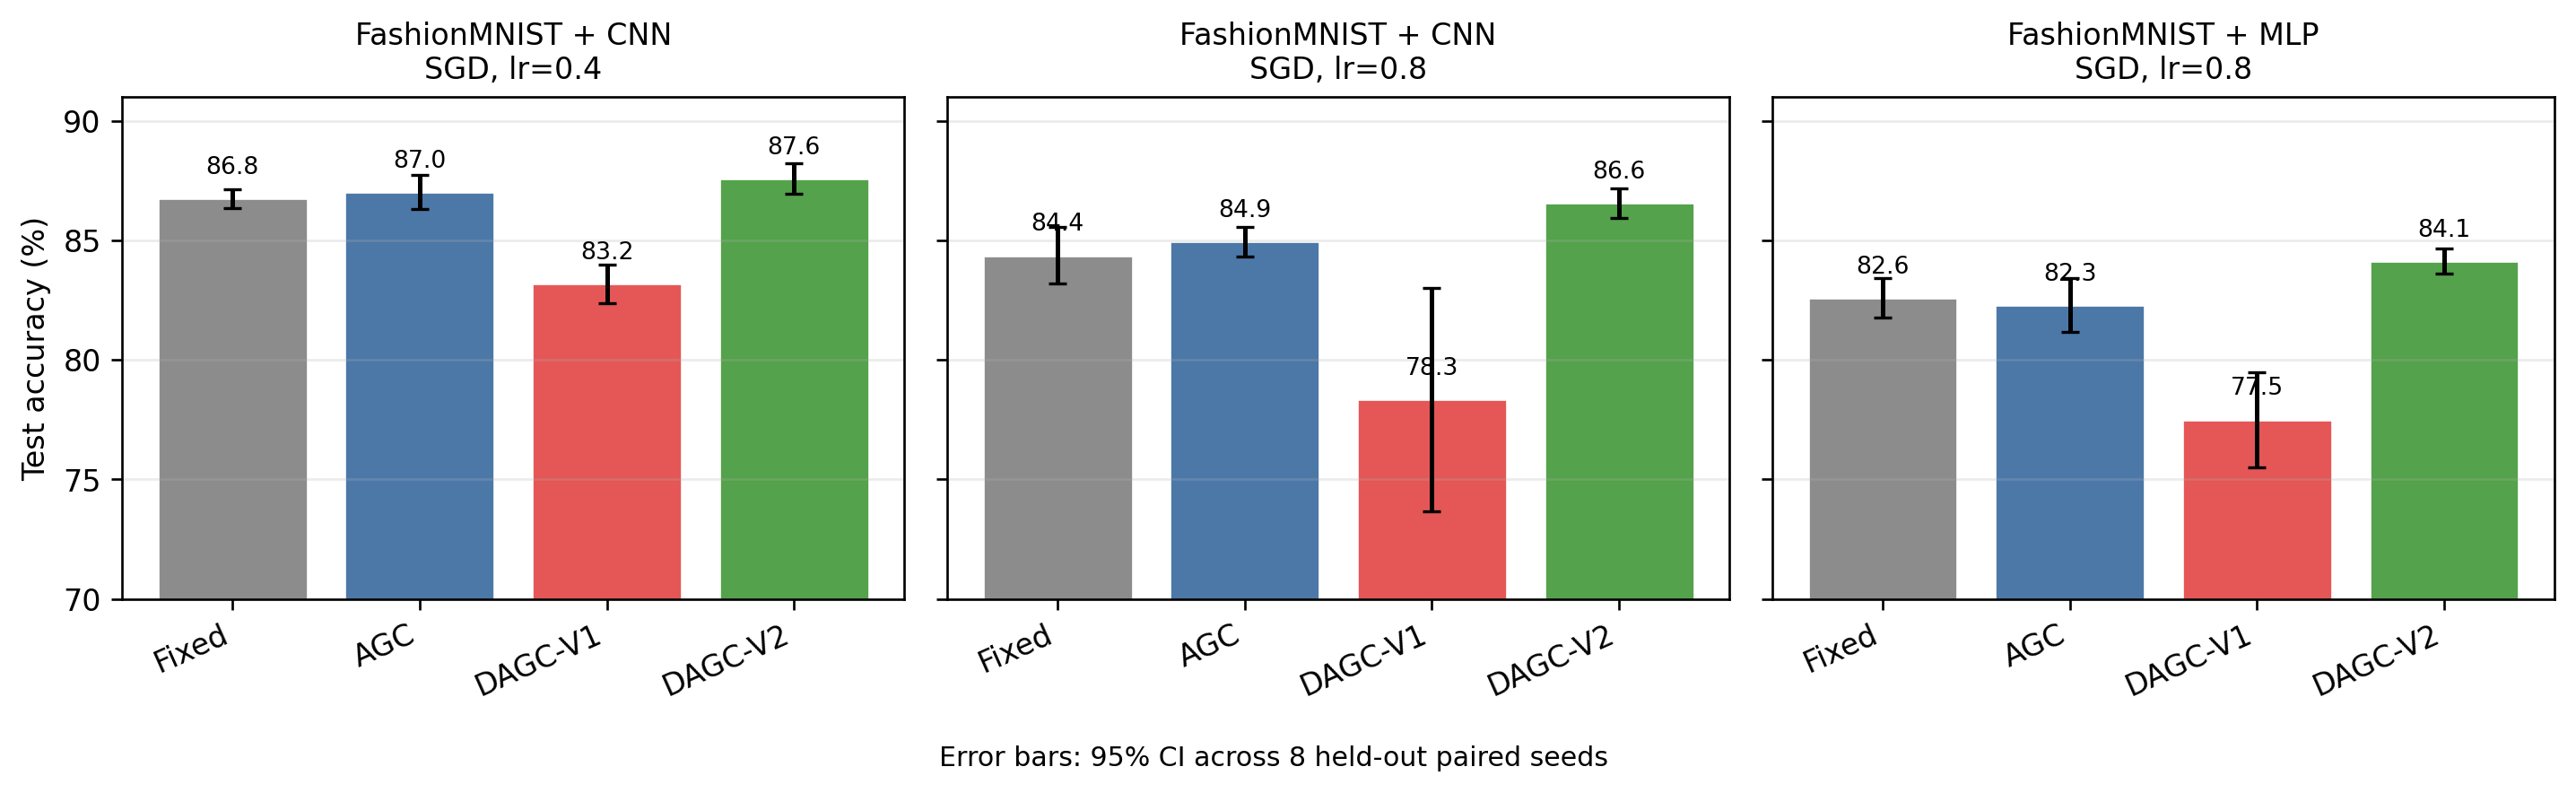
\includegraphics[width=\textwidth]{figures/heldout_accuracy.png}
\caption{Held-out accuracy across the first three unstable-training conditions.
Each bar summarizes eight paired evaluation seeds; error bars are 95\%
confidence intervals. The fixed baseline is separately calibrated in each
condition, while DAGC-V2 remains frozen.}
\label{fig:heldout}
\end{figure*}

The V1 columns expose why the correction matters. V1 is lower than fixed
clipping in all four conditions and has particularly large seed variation at
FashionMNIST-CNN $0.8$ and MNIST-CNN $0.8$. This is consistent with the control
analysis: since the V1 exposure term is non-negative at every exposure level,
heavy clipping alone cannot make the threshold fall, which is consistent with
insufficient protection where
clipping is needed. Its mean realized clipping intensity at FashionMNIST-CNN
$0.8$ is $0.349$, against $0.795$ for V2 ($0.505$ versus $0.810$ on the MLP and
$0.340$ versus $0.433$ on MNIST-CNN), which is the predicted symptom.

\paragraph{What the correction buys, and what it does not.}
Table~\ref{tab:tau} and Figure~\ref{fig:tau} report the development sweep. The
two candidate explanations make different predictions: if V2 worked by driving
realized exposure towards $\tau$, accuracy should depend on $\tau$; if it worked
by letting the threshold fall, accuracy should be insensitive to $\tau$ and
realized exposure should saturate. The data support the second reading. Over a
sevenfold range of $\tau$, from $0.1$ to $0.7$, accuracy moves by $0.68$ points
in total and the five means are mutually overlapping. Realized exposure sits at
$1.000$ for every run up to $\tau=0.5$ and $0.999$ at $\tau=0.7$; at $\tau=0.1$
it exceeds the reference level tenfold and never approaches it. The reference
level therefore sets the sign changeover of the exposure term, not a level the
controller reaches, and what distinguishes V2 from V1 is that the threshold can
decrease at all.

Figure~\ref{fig:tau} draws both halves of that argument. The left panel is the
$\tau$--accuracy curve: it is flat, and the five V2 means lie inside a band
$0.68$ points wide, so any reading in which the controller steers exposure
towards $\tau$ predicts a dependence that is not present. The same panel places
V1 at $\tau=1$, which is not an approximation: the V1 rule is exactly the V2
rule with the reference level at the ceiling, so the two coincide there, as we
verified by running both controllers on a common trajectory. The panel shows the
$+4.8$ point gap that the one-sign change produces against V1 --- roughly seven
times the entire spread across $\tau$. The right panel shows why. Realized
exposure is pinned at the ceiling for every run while the reference level rises
from $0.1$ to $0.7$, so the exposure term stays near saturation and the
controller never receives a signal that would pull it back towards $\tau$.

One systematic trend does survive, and we report it rather than smoothing it
over: mean clipping intensity falls monotonically with $\tau$, from $0.825$ at
$\tau=0.1$ to $0.697$ at $\tau=0.7$. A larger reference level relaxes the
tightening term and so clips somewhat less, exactly as the rule dictates. What
$\tau$ does not do over this range is change the accuracy outcome, which is the
property the tracking reading required.

\begin{figure}[t]
\centering
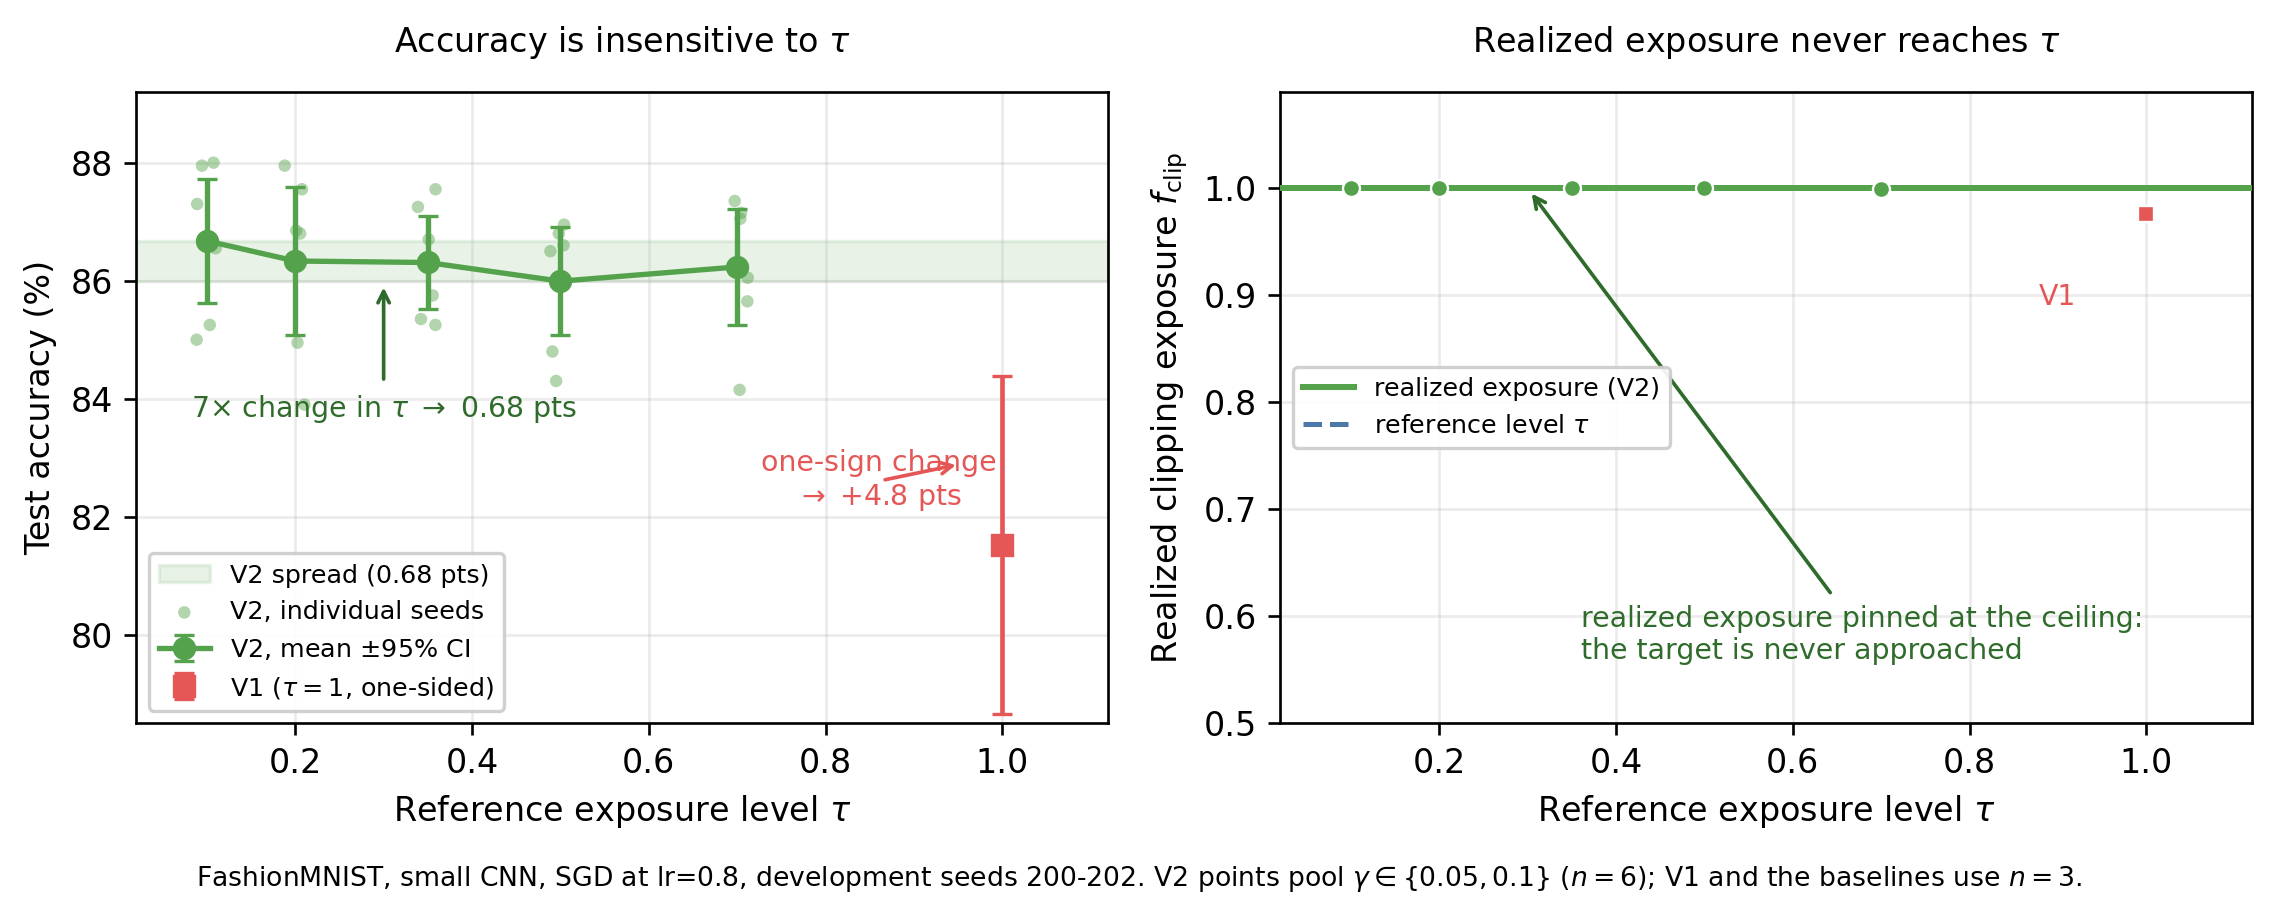
\includegraphics[width=\linewidth]{figures/tau_sweep_accuracy.png}
\caption{The reference exposure level $\tau$ does not control realized exposure.
Left: accuracy against $\tau$ for V2, with individual seeds, means, and 95\%
intervals; the shaded band spans the five V2 means. V1 is placed at $\tau=1$,
the value that exactly reproduces the one-sided rule. Right: realized clipping
exposure against $\tau$, with the reference level itself shown dashed.
Development seeds, FashionMNIST, small CNN, SGD at learning rate $0.8$.}
\label{fig:tau}
\end{figure}

\begin{table}[t]
\centering
\caption{Development sweep of the reference exposure level $\tau$
(FashionMNIST, small CNN, SGD at learning rate $0.8$, seeds 200--202, three
seeds per cell). Each cell pools the two values of $\gamma$ tested
($0.05$ and $0.1$), so $n=6$; accuracy is mean test accuracy with a
normal-approximation 95\% interval. Realized exposure never falls below
$0.999$ and is never near any $\tau$ tested, while mean clipping intensity
decreases monotonically in $\tau$.}
\label{tab:tau}
\small
\begin{tabular}{lcccc}
\toprule
$\tau$ & $n$ & Accuracy (\%) & $f_\text{clip}$ & $i_\text{clip}$ \\
\midrule
$0.10$ & 6 & $86.68 \pm 1.05$ & 1.000 & 0.825 \\
$0.20$ & 6 & $86.33 \pm 1.26$ & 1.000 & 0.809 \\
$0.35$ & 6 & $86.31 \pm 0.79$ & 1.000 & 0.788 \\
$0.50$ & 6 & $85.99 \pm 0.91$ & 1.000 & 0.758 \\
$0.70$ & 6 & $86.23 \pm 0.98$ & 0.999 & 0.697 \\
\midrule
V1 ($\tau=1$)      & 3 & $81.52 \pm 2.87$ & 0.976 & 0.435 \\
Fixed (calibrated) & 3 & $84.13 \pm 1.05$ & 1.000 & 0.695 \\
AGC (published)    & 3 & $84.58 \pm 2.48$ & 1.000 & 0.926 \\
\bottomrule
\end{tabular}
\end{table}

\subsection{Diagnostics and negative controls}
The A3 ablation shows why exposure feedback was retained during controller
development. On the stable FashionMNIST-CNN setting, the original DAGC reaches
$79.38\pm1.20\%$, compared with $77.63\pm1.63\%$ after removing exposure
feedback and $77.67\pm1.64\%$ with a frozen threshold. Removing alignment
feedback gives $78.90\pm0.58\%$. More directly, the exposure and frozen
variants reduce threshold switches from $8.2$ per run to $1.8$ and $1.4$ while
raising clipping intensity from $0.493$ to approximately $0.626$. This is a
behavioural ablation, not evidence of a stable-regime accuracy advantage: its
five seeds are small in number and it precedes V2.

\begin{figure}[t]
\centering
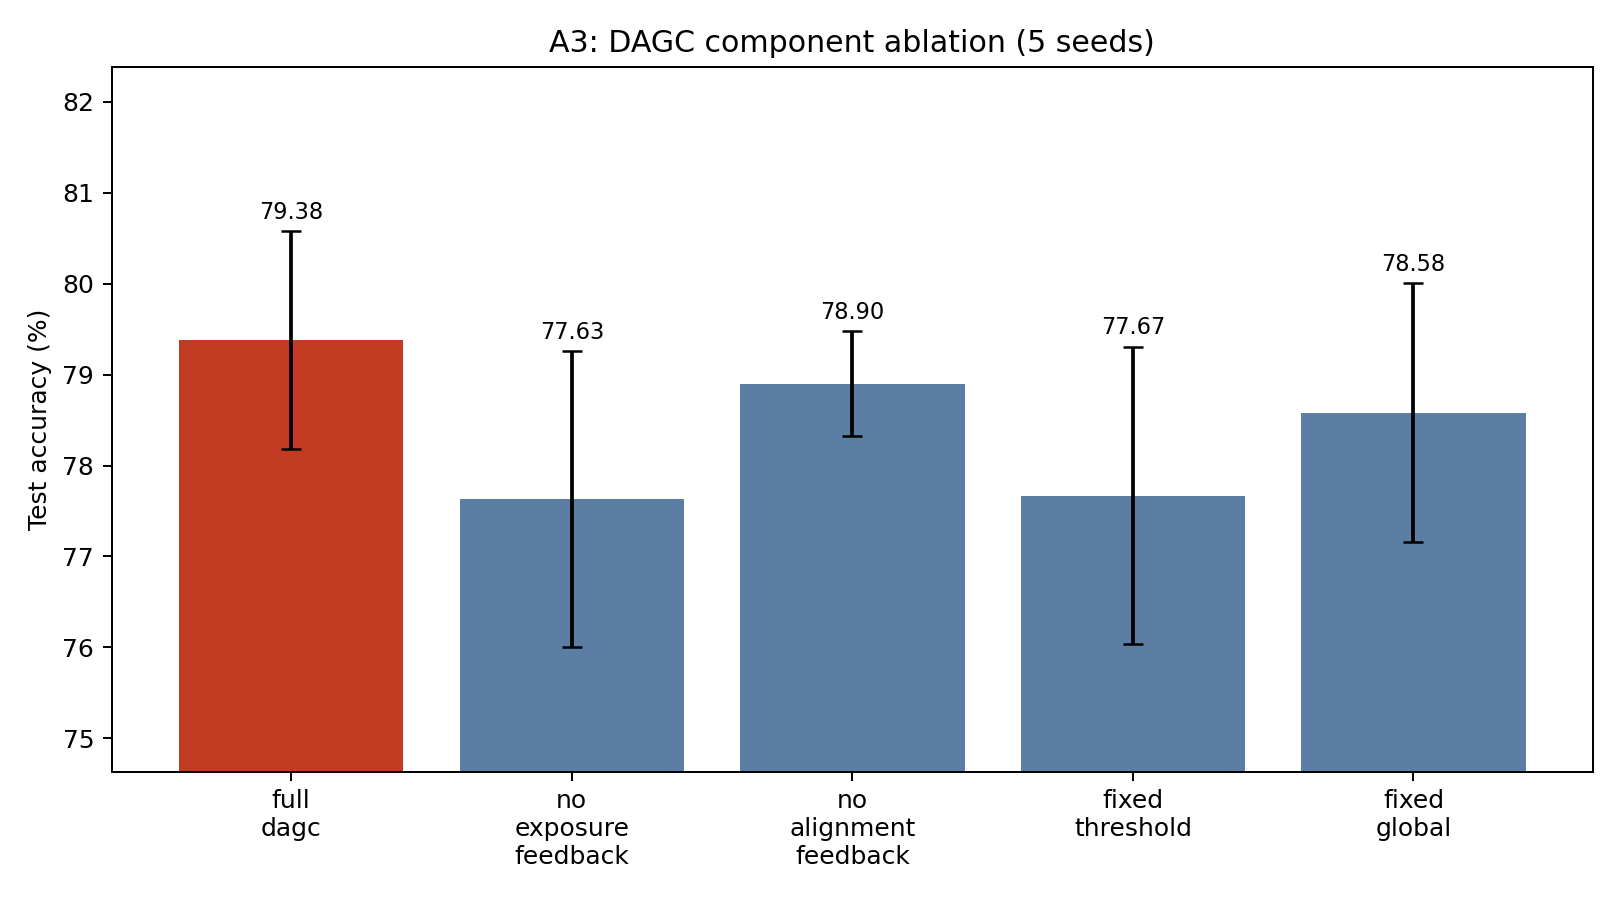
\includegraphics[width=\linewidth]{figures/a3_ablation_accuracy.png}
\caption{A3 diagnostic ablation of the original controller on FashionMNIST-CNN
at a stable learning rate. Error bars summarize five seeds. The experiment
motivates exposure feedback but is not used as a V2 performance claim.}
\label{fig:ablation}
\end{figure}

The A4 grid supplies the complementary negative control. Across all sixteen
dataset-model-optimizer cells at low learning rates, no clipping matches or
exceeds the original DAGC. For example, FashionMNIST-CNN with SGD yields
$82.27\pm1.68\%$ without clipping versus $79.90\pm0.81\%$ with DAGC; MNIST-MLP
with SGD yields $92.82\pm0.56\%$ versus $92.18\pm0.55\%$. The absence of a gain
where the optimizer is already stable is expected and limits the intended claim
to the unstable regime. It also guards against interpreting adaptive clipping
as a universal accuracy improvement.

\subsection{Discriminating mechanism experiments}
We perform a new eight-seed paired experiment on FashionMNIST-CNN at learning
rate $0.8$, retaining the fifteen-epoch protocol. Calibration seeds 800--802
are disjoint from evaluation seeds 900--907. The calibration V2 traces define
an open-loop replay schedule by averaging thresholds at each training step.
A fixed threshold is chosen from $\{0.05,0.10,0.20,0.30,0.50\}$ solely to
minimize the discrepancy in calibration mean clipping intensity; this selects
$0.20$. No evaluation scores select either control.

\begin{table}[t]
\centering
\caption{Mechanism test, eight paired held-out seeds. Accuracy intervals are
normal-approximation 95\% intervals. $I$ is mean clipping intensity.}
\label{tab:mechanism}
\small
\begin{tabular}{lcc}
\toprule
Policy & Accuracy (\%) & $I$ \\
\midrule
Full V2 & $86.79\pm0.55$ & 0.798 \\
No alignment & $86.63\pm0.77$ & 0.790 \\
No exposure & $81.33\pm1.03$ & 0.399 \\
Frozen threshold & $80.74\pm0.86$ & 0.346 \\
Intensity-matched fixed & $85.61\pm0.77$ & 0.762 \\
Calibration-trace replay & $86.58\pm0.46$ & 0.789 \\
AutoClip ($p=0.10$) & $79.88\pm1.44$ & 0.232 \\
Rate tracking & $75.21\pm1.57$ & 0.160 \\
\bottomrule
\end{tabular}
\end{table}

\paragraph{Comparison with the closest feedback mechanisms.}
AutoClip uses the tenth percentile of all gradient norms observed through the
current step. Rate tracking uses the same initial threshold, exposure EMA,
gain, and saturation as V2, but reverses the exposure sign and removes the
direction term: $c^{+}=c\exp[0.05\tanh(0.3(E-0.1))]$. This is a controlled
rate-tracking analogue, not the original private federated algorithm. V2
outperforms these specified configurations by $6.92\pm1.27$ and
$11.59\pm1.63$ paired percentage points, respectively. These configurations
are not comprehensively tuned, so the result distinguishes feedback behaviour
in this regime, rather than establishing method-wide superiority.

\paragraph{Is a smaller threshold sufficient?}
V2 exceeds the calibration-intensity-matched fixed rule by $1.18\pm0.47$
paired points, with seven wins in eight seeds. Evaluation intensities are close
but not identical (0.798 versus 0.762); this finite-grid control is approximate.
Crucially, replaying the calibration threshold trace gives $86.58\%$, and V2's
paired advantage is only $0.21\pm0.53$ points (five wins). Thus a useful
time-varying threshold profile reproduces most of the gain without online
feedback. The experiment does not identify an additional benefit from reacting
to the current evaluation trajectory.

\paragraph{Is the direction signal necessary?}
Removing alignment changes accuracy by only $0.16\pm0.41$ paired points;
V2 wins four comparisons, ties two, and loses two. Removing exposure costs
$5.47\pm1.19$ points, with V2 winning all eight comparisons. These results
support exposure-driven threshold adaptation in this setting, but do not
support necessity of the direction term. An exposure-only controller is a
competitive simplification. Neither comparison establishes that reversal
predicts future loss deterioration.

\subsection{Does online feedback help after a learning-rate change?}
We additionally test two prespecified perturbations using independent paired
seeds 1000--1007. In the pulse condition, the learning rate changes from $0.8$
to $1.6$ immediately before zero-based step 100 and returns to $0.8$ before
step 160. In the drop condition it changes from $0.8$ to $0.2$ before step
100 and remains there. The 300-step budget, data protocol, momentum buffer,
and V2 settings are unchanged. The replay schedule is still the original
unperturbed calibration trace; neither condition recalibrates it.

\begin{table}[t]
\centering
\caption{Learning-rate perturbations: eight paired seeds per policy.}
\label{tab:perturbation}
\small
\setlength{\tabcolsep}{2pt}
\begin{tabular}{lcc}
\toprule
Policy & Pulse accuracy (\%) & Drop accuracy (\%) \\
\midrule
Full V2 & $86.47\pm0.59$ & $86.88\pm0.43$ \\
No alignment & $86.49\pm0.53$ & $86.66\pm0.44$ \\
Trace replay & $86.53\pm0.81$ & $86.87\pm0.65$ \\
\bottomrule
\end{tabular}
\end{table}

V2's paired advantage over replay is $-0.06\pm0.54$ points under the pulse
and $+0.01\pm0.43$ under the drop. Against the no-alignment variant, its
advantage is $-0.02\pm0.43$ and $+0.21\pm0.35$ points, respectively.
Thus neither perturbation identifies additional accuracy benefit from online
feedback or the direction term. These results reject the proposed empirical
discriminator in these settings: the predetermined schedule remains competitive
even after a learning-rate change. They do not show equivalence outside the
tested perturbation magnitudes or training budget.

\section{Discussion and Limitations}
The new controls narrow the mechanism claim. Exposure removal harms performance,
but direction removal does not produce a detectable accuracy change. A
calibration-derived open-loop schedule nearly matches online V2. The current
evidence therefore supports generating a protective threshold profile, not a
unique advantage of real-time direction-sensitive feedback. Distinguishing
these alternatives is part of the contribution of the mechanism experiments.
The evidence supports a narrow claim: under the tested high-learning-rate,
small-data protocols, bidirectional exposure feedback improves the clipped
training outcome over a separately calibrated fixed threshold and AGC. The paired
design, separate fixed-baseline calibration, and frozen V2 setting reduce the
most obvious sources of selection bias. The low-learning-rate diagnostic
benchmark from the development stage remains a negative control: clipping is not
expected to improve accuracy when the unconstrained optimizer is already stable.

One result narrowed our own interpretation. We introduced V2 to track a target
exposure, and the $\tau$ sweep shows it does not: over a sevenfold range
accuracy is flat in $\tau$ and realized exposure saturates at the ceiling, even
though clipping intensity does respond to $\tau$ as the rule dictates. What the
correction reliably provides is a threshold that can decrease, and in the
unstable regime the controller then holds clipping on for essentially every
step. That is a real mechanism, and it explains the V1 failure, but it is not
the mechanism we set out to test, and a reviewer should read the V2 gain as
evidence for permissive-versus-committed threshold control rather than for
target tracking. The dissociation matters for how the hyperparameter should be
tuned: $\tau$ controls how hard the controller clips, not whether the threshold
may fall, so it should be selected for intensity rather than treated as the
quantity the controller regulates. A cleaner test of the tracking hypothesis
would vary $\tau$ together with the learning rate and ask whether a nonzero
$\tau$ ever binds; our sweep suggests it may not in MNIST-family settings.

The limitations are substantial. The present experiments use MNIST-family data,
small CNN/MLP models, short schedules, and normal-approximation intervals with
eight seeds. Only fixed global clipping receives per-condition tuning; AGC is
reported with its standard coefficient rather than an exhaustive tuning budget,
and the same is true of the ZClip and AdaGC baselines, so no claim about those
methods is available from these runs. The V2 controller itself is selected on
one FashionMNIST-CNN configuration, so its apparent transfer must be verified on
larger and more diverse benchmarks. A full submission should add three-channel
datasets, larger architectures, longer schedules, and a matched tuning budget
for every adaptive baseline.

\section{Conclusion}
DAGC-V2 adapts a global clipping threshold through bidirectional exposure
feedback and consecutive-gradient dynamics. Its defining correction over V1 is
simple: making the exposure term change sign allows persistent clipping to
tighten the threshold rather than merely slow its relaxation, and in the tested
regime that is what separates under-clipping from committed clipping. Across
four disjoint held-out evaluations, the frozen controller consistently exceeds
calibrated fixed clipping and AGC. A sweep of the reference level shows the
benefit does not come from tracking a target exposure, and we report it that
way. The new mechanism controls show that exposure-only adaptation and a
calibration-derived schedule capture most of the gain; they do not establish
necessity of directional feedback. These results motivate focused validation, while their
MNIST-family diagnostic scope sets clear limits on the claims that can be made
at present.

\bibliography{references}
\bibliographystyle{icml2026}

\clearpage
\onecolumn
\appendix
\section{Reproducibility Details}
\label{app:reproducibility}
Source code, evaluation scripts, and seed-level experimental artifacts are
available at
\url{https://github.com/alexsongyzs-dotcom/Dynamics_Aware_Gradient_Clipping}.
This public manuscript includes the repository link; an anonymous review copy
should use an anonymized code archive in accordance with the submission rules.
\begin{table}[h]
\centering
\caption{Shared experimental settings. Values not listed are fixed by the
policy definition or the calibration protocol.}
\label{tab:settings}
\small
\begin{tabular}{ll}
\toprule
Setting & Value \\
\midrule
Framework / device & PyTorch / CUDA \\
Optimizer & SGD, momentum $0.9$ \\
Weight decay & $10^{-4}$ \\
Epochs / batch size & $15$ / $256$ \\
Train / test subset & $5{,}000$ / $2{,}000$ \\
Projection dimension & $8$ \\
Divergence loss / jump & $100$ / $\max(50,20\ell_{t-1}+1)$ \\
V2 $(c_0,\gamma,\beta,r,w,\tau)$ & $(0.5,0.05,0.9,0.3,3.0,0.1)$ \\
AGC coefficient / epsilon & $0.01$ / $10^{-3}$ \\
\bottomrule
\end{tabular}
\end{table}

The evaluation code records complete seed-level outcomes in CSV files. The
controller state resets at the beginning of each run. Dataset subsets are
sampled deterministically from a seed, and a separate generator controls the
shuffled batch order. Consequently, policies with different control trajectories
do not accidentally see a different minibatch sequence.

\section{Calibration and Held-Out Splits}
The V2 development sweep uses seeds 200--202 on FashionMNIST-CNN at learning
rate $0.8$. It considers exposure targets $0.10$, $0.20$, and $0.35$ and gains
$\gamma\in\{0.05,0.10\}$, alongside fixed clipping, AGC, and V1. The selected
V2 configuration in Table~\ref{tab:settings} is then not changed. Fixed
clipping thresholds are selected separately on seeds 400--402 for
FashionMNIST-MLP and 600--602 for MNIST-CNN. FashionMNIST-CNN uses an earlier
disjoint calibration run. All reported evaluation seeds are absent from these
development and calibration splits.

This split does not eliminate all selection effects: the unstable learning-rate
band follows an earlier pilot. It does prevent reported evaluation seeds from
selecting the V2 target or fixed threshold. This distinction matters because an
overly restrictive fixed threshold can make an adaptive policy look better for
the wrong reason.

\section{Additional Seed-Level Interpretation}
Paired differences are evaluated within a seed, not by subtracting unpaired
aggregate means. V2 beats calibrated fixed clipping in 6/8, 7/8, 8/8, and 8/8
seeds across the four conditions; it beats AGC in 5/8, 8/8, 8/8, and 8/8. The
smaller 5/8 margin at FashionMNIST-CNN with learning rate $0.4$ is reported
deliberately: it shows the effect is smaller when optimization is less stressed.
The result is directional, rather than an assertion that every unstable setting
benefits equally.

V1 supplies a useful failure case. It remains stable under clipping but
underperforms both fixed clipping and V2 in every held-out condition. This
separates avoiding divergence from preserving useful learning dynamics. The
bidirectional correction allows the controller to reduce its threshold rather
than merely slow the rate at which it increases, and the measured difference in
realized clipping intensity between V1 and V2 in each condition is the direct
trace of that change.
\section{Mechanism Experiment: Complete Protocol}
\label{app:mechanism}
\subsection{Data, architecture, and training budget}
This experiment uses FashionMNIST, normalized with mean $0.286$ and standard
deviation $0.353$. Each seed selects 5,000 training and 2,000 test images
without replacement. Training indices use the run seed; test indices use the
seed plus one. The CNN has two $3\times3$ convolutional layers with 32 and 64
channels, each followed by ReLU and $2\times2$ max pooling. Its classifier is
a flattened $64\times7\times7$ representation, a 128-unit ReLU layer, and a
ten-class output. Cross-entropy is optimized with SGD at constant learning
rate $0.8$, momentum $0.9$, and weight decay $10^{-4}$. Batch size is 256;
there are 20 minibatches per epoch and 300 planned steps over 15 epochs.
Data-loader workers are set to zero. All policies within a seed share subset,
initialization, and shuffled minibatch order.

\subsection{Calibration and frozen controls}
Calibration uses seeds 800--802. We run V2 and five fixed thresholds on each
seed, giving 18 calibration runs. Evaluation uses seeds 900--907 and eight
policies, giving 64 independent evaluation runs. The following choices are
frozen before evaluation.

\paragraph{Intensity matching.}
For step $t$, clipping intensity is
$I_t=\max(0,1-c_t/(\|g_t\|+10^{-12}))$; a run's intensity is its mean over
completed steps. We average run intensities across the three calibration seeds.
The V2 mean is $0.795853$. We choose the fixed threshold minimizing the
absolute discrepancy with this mean, without using accuracy for selection.
The grid and absolute discrepancies are:
\begin{center}
\begin{tabular}{lccccc}
\toprule
Threshold & 0.05 & 0.10 & 0.20 & 0.30 & 0.50 \\
Absolute intensity discrepancy & 0.179211 & 0.123842 & 0.025591 & 0.160509 & 0.383605 \\
\bottomrule
\end{tabular}
\end{center}
This selects $c=0.20$. Matching is approximate, since the grid is finite and
calibration and evaluation seeds differ.

\paragraph{Open-loop replay.}
For each step $t$, the predetermined threshold is
$\bar c_t=\frac13\sum_{s=800}^{802}c_{s,t}^{\mathrm{V2}}$.
We average the thresholds actually applied to that step, not their next-step
values. Evaluation replays this 300-step schedule without observing gradient
norms or directions to select the threshold; the current norm is used only to
apply clipping. The schedule is constructed solely from calibration runs and
is shared by all evaluation seeds.

\subsection{Exact policy definitions}
\begin{description}
\item[Full V2.] $c_0=0.5$, $\gamma=0.05$, exposure and alignment EMA decay
both $0.9$, exposure gain $r=0.3$, alignment gain $w=3$, and reference
$\tau=0.1$. The running norm window is 200 steps. Bounds are $0.1$ and $10$
times the rolling median, with numerical floors $10^{-12}$ and $10^{-9}$.
Exposure state starts at zero and alignment state at one.
\item[No alignment.] Full V2 with $w=0$; all other settings remain equal.
\item[No exposure.] Full V2 with $r=0$; alignment and scale bounds remain active.
\item[Frozen threshold.] Full V2 with $\gamma=0$. This disables the
multiplicative update, but the running scale projection remains active, so it
is not strictly constant. The genuinely constant control is the fixed rule.
\item[Intensity-matched fixed.] Constant global threshold $c=0.20$.
\item[Calibration-trace replay.] Apply the predetermined $\bar c_t$ above.
\item[AutoClip.] At step $t$, compute the empirical tenth percentile of all
raw gradient norms from steps 1 through $t$, including the current norm, and
apply it as the threshold. There is no warmup or moving-window truncation.
\item[Rate tracking.] Initial threshold $0.5$, exposure EMA initialized at
zero with decay $0.9$, reference $0.1$, and update
$c_{t+1}=c_t\exp[0.05\tanh(0.3(E_t-0.1))]$ after applying $c_t$.
There is no alignment penalty or rolling-median projection. This is a
specified non-private tracking analogue, not a reproduction of DP-FedAvg.
\end{description}
AutoClip and rate tracking use prespecified settings without a matched
hyperparameter search. Their results should be interpreted as configuration
comparisons. The frozen variant retains scale adaptation through its bounds;
its name does not imply that every source of threshold movement is removed.

\subsection{Logging, evaluation, and statistical analysis}
We store per-step loss, raw gradient norm, clipping coefficient, actual parameter
update norm, consecutive full-gradient alignment, exposure, intensity, signed
threshold crossing, and applied threshold. Alignment used by the controller is
computed from the full flattened gradients; the eight-dimensional fixed random
projection is used for additional diagnostics. A divergent run is flagged for
nonfinite loss or gradient norm, loss above 100, or
$\ell_t>\max(50,20\ell_{t-1}+1)$ for a finite previous loss. Final test accuracy is measured after
training and retained for all runs, including flagged runs.

For each alternative $b$, we compute
$d_s=100(\mathrm{accuracy}_{s,\mathrm{V2}}-\mathrm{accuracy}_{s,b})$ for
each of the eight seeds. We report $\bar d\pm1.96s_d/\sqrt8$, count strict
positive differences as wins, and count exact equal scores separately as ties.
These are descriptive normal-approximation intervals, not multiplicity-adjusted
hypothesis tests. No step-level measurements are treated as independent
accuracy replicates.

\subsection{Reproduction and saved artifacts}
From the experimental repository root, run
\begin{quote}
\texttt{python scripts/run\_v2\_mechanism.py}
\end{quote}
Outputs are written to \texttt{results/v2\_mechanism/}. Each calibration and
evaluation run has a JSON file containing its summary and complete trajectory.
\texttt{frozen\_protocol.json} records the seeds, intensity matching errors,
selected fixed threshold, and replay schedule. \texttt{raw\_runs.csv} contains
the 64 evaluation rows; \texttt{summary.csv} contains aggregate and paired
statistics. Existing per-run JSON files are reused when resuming. Files must
be moved to a fresh output location before changing the protocol, since cached
results are not automatically invalidated by configuration edits.
\section{Learning-Rate Perturbation Reproduction}
Run \texttt{python scripts/run\_v2\_lr\_perturbation.py}. The script records
the two perturbation schedules and seeds in
\texttt{results/v2\_lr\_perturbation/protocol.json}. Each of the 48 runs
has a trajectory JSON, and \texttt{raw\_runs.csv} and \texttt{summary.csv}
contain final outcomes and paired comparisons. Step indices are zero-based;
learning-rate changes occur before the indicated batch's forward pass, with
the momentum state retained. The original calibration replay schedule is read
from \texttt{results/v2\_mechanism/frozen\_protocol.json}. V2, no alignment,
and replay are compared under the same perturbation within each seed. No new
controller parameters or replay traces are selected using these evaluations.
\end{document}
